\documentclass[xcolor=pdflatex,dvipsnames,table]{beamer}
\usepackage{epsfig,graphicx}
\usepackage{palatino}
\usepackage{fancybox}
\usepackage{relsize}
\usepackage[procnames]{listings}
\usepackage{array}

% "define" Scala
\usepackage[T1]{fontenc}  
\usepackage[scaled=0.82]{beramono}  
\usepackage{microtype} 

\sbox0{\small\ttfamily A}
\edef\mybasewidth{\the\wd0 }

\lstdefinelanguage{scala}{
  morekeywords={abstract,case,catch,class,def,%
    do,else,extends,false,final,finally,%
    for,if,implicit,import,match,mixin,%
    new,null,object,override,package,%
    private,protected,requires,return,sealed,%
    super,this,throw,trait,true,try,%
    type,val,var,while,with,yield},
  sensitive=true,
  morecomment=[l]{//},
  morecomment=[n]{/*}{*/},
  morestring=[b]",
  morestring=[b]',
  morestring=[b]"""
}

\usepackage{color}
\definecolor{dkgreen}{rgb}{0,0.6,0}
\definecolor{gray}{rgb}{0.5,0.5,0.5}
\definecolor{mauve}{rgb}{0.58,0,0.82}

% Default settings for code listings
\lstset{frame=tb,
  language=scala,
  aboveskip=3mm,
  belowskip=3mm,
  showstringspaces=false,
  columns=fixed, % basewidth=\mybasewidth,
  basicstyle={\small\ttfamily},
  numbers=none,
  numberstyle=\footnotesize\color{gray},
  % identifierstyle=\color{red},
  keywordstyle=\color{blue},
  commentstyle=\color{dkgreen},
  stringstyle=\color{mauve},
  frame=single,
  breaklines=true,
  breakatwhitespace=true,
  procnamekeys={def, val, var, class, trait, object, extends},
  procnamestyle=\ttfamily\color{red},
  tabsize=2
}

\lstnewenvironment{scala}[1][]
{\lstset{language=scala,#1}}
{}
\lstnewenvironment{cpp}[1][]
{\lstset{language=C++,#1}}
{}
\lstnewenvironment{bash}[1][]
{\lstset{language=bash,#1}}
{}
\lstnewenvironment{verilog}[1][]
{\lstset{language=verilog,#1}}
{}


\lstset{basicstyle={\footnotesize\ttfamily}}

\usetheme[height=8mm]{Rochester}
\setbeamersize{text margin left=3mm} 
\setbeamersize{text margin right=3mm} 
\setbeamertemplate{navigation symbols}{}

\definecolor{Cobalt}{rgb}{0.25,0.125,0.70}
\definecolor{RedOrange}{rgb}{0.8,0.25,0.0}
% \definecolor{RedOrange}{rgb}{0.8,0.775,0.25}
\def\frametitledefaultcolor{Cobalt}
\def\frametitleproblemcolor{RedOrange}

\lstset{basicstyle={\footnotesize\ttfamily}}

\setbeamertemplate{frametitle}
{
\vskip-7mm
\textbf{\insertframetitle}\hfill\insertframenumber
}
\setbeamercolor{frametitle}{bg=\frametitledefaultcolor}

\newenvironment{sample}{\VerbatimEnvironment\begin{footnotesize}\begin{semiverbatim}}{\end{semiverbatim}\end{footnotesize}}

\newenvironment{FramedSemiVerb}%
{\begin{Sbox}\begin{minipage}{.94\textwidth}\begin{semiverbatim}}%
{\end{semiverbatim}\end{minipage}\end{Sbox}
\setlength{\fboxsep}{8pt}\fbox{\TheSbox}}

\newenvironment{FramedVerb}%
{\VerbatimEnvironment
\begin{Sbox}\begin{minipage}{.94\textwidth}\begin{Verbatim}}%
{\end{Verbatim}\end{minipage}\end{Sbox}
\setlength{\fboxsep}{8pt}\fbox{\TheSbox}}

% \newenvironment{sample}{\VerbatimEnvironment\begin{footnotesize}\begin{Verbatim}}{\end{Verbatim}\end{footnotesize}}
\newcommand{\code}[1]{\begin{footnotesize}{\tt #1}\end{footnotesize}}
\newcommand{\comment}[1]{{\color{Green}\it\smaller #1}}


\title[Chisel]{Chisel: Constructing Hardware In a Scala Embedded Language}
\author[Bachrach et al]{Jonathan Bachrach, Huy Vo, Brian Richards, \\
Yunsup Lee, Andrew Waterman, Rimas Avizienis, Henry Cook, \\
John Wawrzynek, Krste Asanovic}
\date{\today}
\institute[parlab]{EECS UC Berkeley}

\begin{document}

{
\setbeamertemplate{footline}{} 
\begin{frame}
  \titlepage
\end{frame}
}
\addtocounter{framenumber}{-1}

\begin{frame}[fragile]
\frametitle{21st Century Architecture Design}
{\Large\textbf{Harder to get hardware / software efficiency gains}}
\vskip5mm
\begin{itemize}
\item Need massive design-space exploration
\begin{itemize}
\item Hardware and software codesign and cotuning
\end{itemize}
\item Need meaningful results
\begin{itemize}
\item Cycle counts
\item Cycle time, power and area
\item Real chips
\end{itemize}
\item Traditional architectural simulators, hardware-description
  languages, and tools are inadequate
\begin{itemize}
\item Slow
\item Inaccurate
\item Error prone
\item Difficult to modify and parameterize
\end{itemize}
\end{itemize}
\end{frame}

\begin{frame}[fragile]
\frametitle{Bottom Line -- Shorten Design Loop}
{\LARGE\textbf{Make it}}
\vskip2mm
\begin{itemize}
\item Easier to make design changes
\begin{itemize}
\item Fewer lines of design code ( \textbf{>> 3x} )
\item More reusable code
\item Parameterize designs
\end{itemize}
\item Faster to test results ( \textbf{>> 8x} )
\begin{itemize}
\item Fast compilation
\item Fast simulation
\item Easy testing
\item Easy verification
\end{itemize}
\end{itemize}
\vskip0.8cm
{\LARGE\textbf{Result}}
\begin{itemize}
\item Explore more design space
\end{itemize}

\end{frame}

\begin{frame}[fragile]
\frametitle{Chisel is ...}

\begin{columns}[c]

\column{0.55\textwidth}

\begin{itemize}
\item Best of hardware and software design ideas
\item Embedded within Scala language to leverage mindshare and language design
\item Algebraic construction and wiring
\item Hierarchical, object oriented, and functional construction
\item Abstract data types and interfaces
\item Bulk connections
\item Multiple targets
\begin{itemize}
\item Simulation and synthesis
\item Memory IP is target-specific
\end{itemize}
\end{itemize}

\column{0.40\textwidth}

\begin{center}
single source \\
\includegraphics[width=0.99\textwidth]{../manual/figs/targets.pdf} \\
multiple targets \\
\end{center}

\end{columns}

\end{frame}

\begin{frame}[fragile]
\frametitle{The Scala Programming Language}

\begin{columns}[c]

\column{0.75\textwidth}

\begin{itemize}
\item Compiled to JVM
\begin{itemize}
\item Good performance
\item Great Java interoperability
\item Mature debugging, execution environments
\end{itemize}
\item Object Oriented
\begin{itemize}
\item Factory Objects, Classes
\item Traits, overloading etc
\end{itemize}
\item Functional
\begin{itemize}
\item Higher order functions
\item Anonymous functions
\item Currying etc
\end{itemize}
\item Extensible
\begin{itemize}
\item Domain Specific Languages (DSLs)
\end{itemize}
\end{itemize}

\column{0.25\textwidth}

\begin{center}
\includegraphics[height=0.4\textheight]{figs/programming-scala.pdf} \\
\includegraphics[height=0.4\textheight]{figs/programming-in-scala.pdf}
\end{center}

\end{columns}
\end{frame}

\begin{frame}[fragile]
\frametitle{Algebraic Graph Construction}

\begin{columns}
\column{0.35\textwidth}
{\lstset{basicstyle={\Large\ttfamily}}
\begin{scala}
Mux(x > y, x, y)
\end{scala}
}

\column{0.6\textwidth}

\begin{center}
\includegraphics[width=0.9\textwidth]{figs/max2.pdf} 
\end{center}
\end{columns}
\end{frame}

\begin{frame}[fragile]
\frametitle{Creating Component}

\begin{columns}
\column{0.45\textwidth}

{\lstset{basicstyle={\scriptsize\ttfamily}}
\begin{scala}
class Max2 extends Component {
  val io = new Bundle {
    val x = UFix(width = 8).asInput
    val y = UFix(width = 8).asInput
    val z = UFix(width = 8).asOutput }
  io.z := Mux(io.x > io.y, io.x, io.y)
}
\end{scala}
}

\column{0.45\textwidth}
\begin{center}
\includegraphics[width=0.95\textwidth]{figs/Max2c.pdf} \\
\end{center}
\end{columns}

\end{frame}

\begin{frame}[fragile]
\frametitle{Connecting Components}

\begin{columns}
\column{0.25\textwidth}
\begin{scala}
val m1 = new Max2()
m1.io.x := a
m1.io.y := b
val m2 = new Max2()
m2.io.x := c
m2.io.y := d
val m3 = new Max2()
m3.io.x := m1.io.z
m3.io.y := m2.io.z
\end{scala}

\column{0.7\textwidth}

\begin{center}
\includegraphics[width=0.99\textwidth]{figs/Max4.pdf} \\
\end{center}
\end{columns}

\end{frame}


\begin{frame}[fragile]
\frametitle{Defining Construction Functions}

\begin{columns}

\column{0.45\textwidth}

\begin{scala}
def Max2 = Mux(x > y, x, y)
\end{scala}
\begin{scala}
Max2(x, y)
\end{scala}

\column{0.5\textwidth}

\begin{center}
\includegraphics[width=0.95\textwidth]{figs/Max2.pdf} \\[1cm]
\end{center}

\end{columns}

\end{frame}

\begin{frame}[fragile]
\frametitle{Functional Construction}

\begin{columns}

\column{0.45\textwidth}

\begin{scala}
Reduce(Array(a, b, c, d), Max2)
\end{scala}

\column{0.5\textwidth}

\begin{center}
\includegraphics[width=0.99\textwidth]{figs/reduceMax.pdf} \\
\end{center}

\end{columns}

\end{frame}

\begin{frame}[fragile]
\frametitle{Example}
\begin{columns}

\column{0.45\textwidth}

\begin{footnotesize}
\begin{scala}
class GCD extends Component {
  val io = new Bundle {
    val a     = UFix(INPUT, 16)
    val b     = UFix(INPUT, 16)
    val z     = UFix(OUTPUT, 16)
    val valid = Bool(OUTPUT) }
  val x = Reg(resetVal = io.a)
  val y = Reg(resetVal = io.b)
  when (x > y) {
    x := x - y
  } .otherwise {
    y := y - x
  }
  io.z     := x
  io.valid := y === UFix(0)
}
\end{scala}
\end{footnotesize}

\column{0.45\textwidth}

\begin{center}
\includegraphics[width=0.9\textwidth]{figs/gcd.pdf} 
\end{center}

\end{columns}
\end{frame}

\begin{frame}[fragile]
\frametitle{Primitive Datatypes}
\begin{itemize}
\item{Chisel has 4 primitive datatypes}
\begin{description}
\item[Bits]  -- raw collection of bits
\item[Fix]   -- signed fixed-point number
\item[UFix] -- unsigned fixed-point number
\item[Bool] -- Boolean value
\end{description}
\item Can do arithmetic and logic with these datatypes
\end{itemize}

\textbf{Example Literal Constructions}
\begin{scala}
val sel = Bool(false)
val a   = UFix(25)
val b   = Fix(-35)
\end{scala}
where \verb+val+ is a Scala keyword used to declare variables whose values won't change
\end{frame}

\begin{frame}[fragile]
\frametitle{Aggregate Data Types}

\textbf{Bundle}

\begin{itemize}
\item User-extensible collection of values with named fields
\item Similar to structs
\end{itemize}

\begin{footnotesize}
% \textbf{Bundle Example}
\begin{scala}
class MyFloat extends Bundle{
  val sign        = Bool()
  val exponent    = UFix(width=8)
  val significand = UFix(width=23)
}
\end{scala}
\end{footnotesize}

\textbf{Vec}

\begin{itemize}
\item Create indexable collection of values
\item Similar to arrays
\end{itemize}

\begin{footnotesize}
% \textbf{Vec Example}
\begin{scala}
val myVec = Vec(5){ Fix(width=23) }
\end{scala}
\end{footnotesize}

\end{frame}


\begin{frame}[fragile]
\frametitle{Abstract Data Types}
\begin{itemize}
\item The user can construct new data types
\begin{itemize}
\item Allows for compact, readable code
\end{itemize}
\item Example: Complex numbers
\begin{itemize}
\item Useful for FFT, Correlator, other DSP
\item Define arithmetic on complex numbers
\end{itemize}
\end{itemize}

\begin{footnotesize}
\begin{scala}
class Complex(val real: Fix, val imag: Fix) 
    extends Bundle {
  def + (b: Complex): Complex = 
    new Complex(real + b.real, imag + b.imag)
  ...
}
val a = new Complex(Fix(32), Fix(-16))
val b = new Complex(Fix(-15), Fix(21))
val c = a + b
\end{scala}
\end{footnotesize}

\end{frame}

\begin{frame}[fragile]
\frametitle{Polymorphism and Parameterization}
\begin{itemize}
\item Chisel users can define their own parameterized functions
\begin{itemize}
\item Parameterization encourages reusability
\item Data types can be inferred and propagated
\end{itemize}
\end{itemize}

\textbf{Example Shift Register:}
\begin{scala}
def delay[T <: Data](x: T, n: Int): T = 
  if(n == 0) x else Reg(delay(x, n - 1))
\end{scala}
where
\begin{itemize}
\item The input \verb+x+ is delayed n cycles
\item \verb+x+ can by of any type that extends from \verb+Data+
\end{itemize}

\end{frame}

\begin{frame}[fragile, shrink]
\frametitle{Functional Composition}

% \begin{itemize}
% \item natural
% \item reusable
% \item composable
% \end{itemize}
% \vskip1cm

\begin{Large}
\begin{columns}

\column{0.45\textwidth}
\verb+Map(ins, x => x * y)+ \\
\begin{center}
\includegraphics[height=0.6\textheight]{figs/map.pdf} \\[2cm]
\end{center}

\column{0.45\textwidth}
\verb+Chain(n, in, x => f(x))+ \\
\begin{center}
\includegraphics[width=0.9\textwidth]{figs/chain.pdf} \\
\end{center}

\verb+Reduce(data, Max)+ \\
\begin{center}
\includegraphics[width=0.9\textwidth]{figs/reduce.pdf} \\
\end{center}


\end{columns}

\end{Large}

\end{frame}

% \begin{frame}[fragile, shrink]
% \frametitle{Chain}
% 
% \begin{columns}
% 
% \column{0.6\textwidth}
% 
% \begin{scala}
% def Chain[T <: Data]
%       (n: Int, in: T, f: T => T): T = {
%   if (n == 1)
%     in
%   else 
%    chain(n-1, f(in), f)
% }
% \end{scala}
% usage:
% \begin{scala}
% Chain(n, in, x => x + x)
% \end{scala}
% 
% \column{0.3\textwidth}
% 
% \begin{center}
% \includegraphics[width=0.9\textwidth]{figs/chain.pdf} \\
% \end{center}
% 
% \end{columns}
% \end{frame}
% 
% \begin{frame}[fragile, shrink]
% \frametitle{Map}
% 
% \begin{columns}
% 
% \column{0.6\textwidth}
% 
% \begin{scala}
% def Map[S <: Data, T <: Data]
%       (ins: Seq[T], f: S => T): T
% \end{scala}
% usage:
% \begin{scala}
% Map(ins, h => Reg(h * Reg(x)))
% \end{scala}
%  
% \column{0.3\textwidth}
% 
% \begin{center}
% \includegraphics[height=0.7\textheight]{figs/map.pdf} \\
% \end{center}
% 
% \end{columns}
% \end{frame}
%  
% \begin{frame}[fragile, shrink]{Reduce}
% 
% \begin{columns}
% 
% \column{0.6\textwidth}
% 
% \begin{scala}
% def Reduce[T <: Data]
%       (ins: Seq[T], f: (T, T) => T): T = {
%   val len = ins.length
%   if (len == 1)
%     ins(0)
%   else 
%     f(Reduce(in.slice(0, len/2),   f), 
%       Reduce(in.slice(len/2, len), f))
% }
% \end{scala}
% usage:
% \begin{scala}
% def Max[T <: Num](x: T, y: T) = 
%   Mux(x > y, x, y)
% Reduce(data, Max)
% \end{scala}
% 
% \column{0.3\textwidth}
% 
% \begin{center}
% \includegraphics[width=0.9\textwidth]{figs/Reduce.pdf} \\
% \end{center}
% 
% \end{columns}
% 
% \end{frame}

\begin{frame}[fragile]
\frametitle{Generator}
\begin{footnotesize}
\begin{scala}
class Cache(cache_type:    Int = DIR_MAPPED,
            associativity: Int = 1,
            line_size:     Int = 128,
            cache_depth:   Int = 16,
            write_policy:  Int = WRITE_THRU
           ) extends Component {
  val io = new Bundle() {
    val cpu = new IoCacheToCPU()
    val mem = new IoCacheToMem().flip()
  }
  val addr_idx_width = log2(cache_depth).toInt
  val addr_off_width = log2(line_size/32).toInt
  val addr_tag_width = 32 - addr_idx_width - addr_off_width - 2
  val log2_assoc     = log2(associativity).toInt
  ...
  if (cache_type == DIR_MAPPED)
    ...
\end{scala}
\end{footnotesize}

\end{frame}

\begin{frame}[fragile]
\frametitle{State Elements}

Simplest element is positive edge triggered register:
\begin{scala}
val prev_in = Reg(in)
\end{scala}
Can assign data input later using wiring
\begin{scala}
val pc = Reg(){ UFix(width = 16) }
pc := pc + UFix(1, 16)
\end{scala}
Can quickly define more useful circuits
\begin{scala}
def risingEdge(x: Bool) = x && !Reg(x)
\end{scala}

\end{frame}

\begin{frame}[fragile]
\frametitle{Conditional Updates}

\begin{columns}

\column{0.45\textwidth}

Convenient to specify updates spread across several statements
\begin{scala}
val r = Reg() { UFix(width = 16) } 
when (c === UFix(0)) {
  r := r + UFix(1)
}
\end{scala}
or
{\lstset{frame=shadowbox}
\begin{scala}
when (c1) { r := e1 } 
when (c2) { r := e2 }
\end{scala}
}

\column{0.45\textwidth}

\shadowbox{
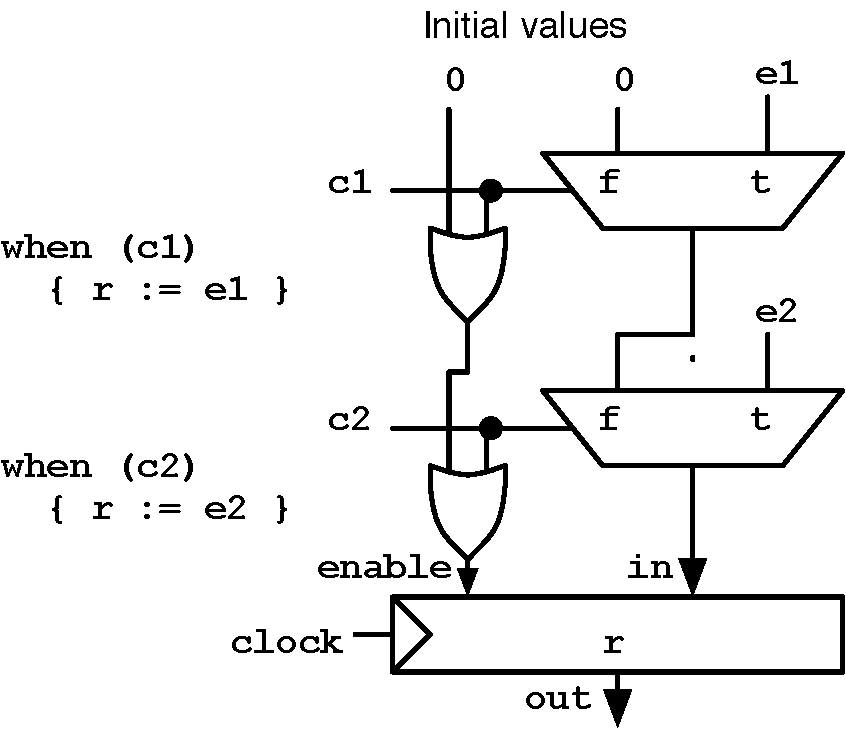
\includegraphics[width=0.95\textwidth]{figs/condupdates.pdf} }

\end{columns}
\end{frame}

\begin{frame}[fragile]
\frametitle{Composition of Conditional Updates}

Nesting
\begin{scala}
when (a) { when (b) { body } }
\end{scala}
Chaining
\begin{scala}
when (c1) { u1 }
.elsewhen (c2) { u2 }
.otherwise { ud }
\end{scala}
Dynamic Scoping
\begin{scala}
def condUpdateR (c: Bool, d: Data) = when (c) { r := d }
\end{scala}
\begin{scala}
when (a) { condUpdateR(b, x) }
\end{scala}
\begin{scala}
when (a) { when (b) { r := x } }
\end{scala}

\end{frame}

\begin{frame}[fragile]
\frametitle{Symmetry of Conditional Updates}

Regs and Wires
\begin{scala}
x := init
when (isEnable) {
  x := data
}
\end{scala}
 
Vecs and Mems
\begin{scala}
when (isEnable) {
  m(addr) := data
}
\end{scala}

\end{frame}

\begin{frame}[fragile]
\frametitle{Object Oriented Conditional Updates}

% \begin{scala}
% class DecoupledIO[T <: Data]()(gen: => T) extends Bundle {
%   val valid = Bool(dir = OUTPUT)
%   val ready = Bool(dir = INPUT)
%   val data  = gen.asOutput
% }
% 
% class EnqIO[T <: Data]()(gen: => T) extends DecoupledIO[T]()(gen) {
%   def enq(dat: T): T = { valid := Bool(true); data := dat; dat }
%   valid := Bool(false)
% }
% 
% class Packet extends Bundle {
%   val header = UFix(width = 8)
%   val body   = Bits(width = 64)
% }
% \end{scala}
% 
% example:

\begin{columns}
\column{0.57\textwidth}

{\lstset{basicstyle={\scriptsize\ttfamily}}
\begin{scala}
val in  = (new DeqIo()){ new Packet() }
val out = (new EnqIo()){ new Packet() }
when (in.valid && out.ready) {
  out.enq(filter(in.deq()))
}
\end{scala}

\vskip5mm

\begin{scala}
val in   = (new DeqIo()){ new Packet() }
val outs = Vec(4){ new EnqIo()){ new Packet() } }
val tbl  = Mem(4){ UFix(width = 2) }
when (in.valid) {
  val k = tbl(in.data.header)
  when (outs(k).ready) {
    outs(k).enq(in.deq())
  }
}
\end{scala}
}

\column{0.38\textwidth}

\includegraphics[width=0.99\textwidth]{figs/filter.pdf} \\[20mm]
\includegraphics[width=0.99\textwidth]{figs/router.pdf} 

\end{columns}

\end{frame}

\begin{frame}[fragile]
\frametitle{Component Testing}

% \begin{itemize}
% \item write tests in Scala
% \item bind values using dot notation
% \end{itemize}

\begin{columns}
\column{0.45\textwidth}

{\lstset{basicstyle={\scriptsize\ttfamily}}
\begin{scala}
class Mux2IO extends Bundle {
  val sel = Bits(width = 1).asInput
  val in0 = Bits(width = 1).asInput
  val in1 = Bits(width = 1).asInput
  val out = Bits(width = 1).asOutput
}
\end{scala}
}
\begin{center}
\includegraphics[width=0.9\textwidth]{figs/mux2.pdf} 
\end{center}

\column{0.5\textwidth}
{\lstset{basicstyle={\scriptsize\ttfamily}}
\begin{scala}
class Mux2Tests extends Iterator[Mux2IO] { 
  var i = 0
  val n = pow(2, 3)
  def hasNext = i < n
  def next = { 
    val io  = new Mux2IO
    val k   = Bits(i, width = log2up(n))
    io.sel := k(0)
    io.in0 := k(1)
    io.in1 := k(2)
    io.out := Mux(k(0), k(1), k(2))
    i      += 1
    io
  }
}
\end{scala}
}

\end{columns}

\end{frame}

\begin{frame}[fragile]
\frametitle{Chisel Line Count Breakdown}

\begin{columns}

\column{0.3\textwidth}

\begin{itemize}
\item \verb+~+5200 lines total
\item Embeds into Scala well
\end{itemize}

\column{0.7\textwidth}

\begin{center}
\includegraphics[width=0.9\textwidth]{figs/linecount.png}
\end{center}

\end{columns}

\end{frame}

\begin{frame}
\frametitle {Chisel versus Hand-Coded Verilog}

\begin{itemize}
\item 3-stage RISCV CPU hand-coded in Verilog
\item Translated to Chisel
\item Resulted in 3x reduction in lines of code
\item Most savings in wiring
\item Lots more savings to go ...
% \item Chisel-generated Verilog gives comparable synthesis quality of results
\end{itemize}

\end{frame}

\begin{frame}[fragile]
\frametitle{Process Language}

\begin{columns}

\column{0.5\textwidth}

Composeable State Machines
\begin{scala}
Do{ ... }
Exec(c){ a } / Exec{ a }
Stop
Skip / Wait(n)
Seq(a, ...)
Par(a, ...)
Alt(c, a1, a2)
While(c){ a } / Loop{ a }
\end{scala}

Each process block uses a \verb+when+
\begin{scala}
when (io.start) { ... }
\end{scala}
to ensure that state updates are updated only when process execute.

\column{0.45\textwidth}

\begin{center}
\includegraphics[width=0.9\textwidth]{figs/process.pdf} \\
\end{center}

\end{columns}

\end{frame}

\begin{frame}[fragile, shrink]
\frametitle{Process Language Example}

\begin{scala}
class Multiply extends Component {
  val io = new Bundle{ 
    val start  = Bool(INPUT);
    val x      = UFix(dir = INPUT, width = 32)
    val y      = UFix(dir = INPUT, width = 32)
    val z      = UFix(dir = OUTPUT, width = 32)
    val finish = Bool(OUTPUT) }
  val a   = Reg(){ UFix(0, 32) }
  val b   = Reg(){ UFix(0, 32) }
  val acc = Reg(){ UFix(0, 32) }
  val finish =
    Exec(io.start) {
      Seq(Do{ a := io.x; b := io.y; acc := UFix(0, 32) },
          While(b != UFix(0, 32)) {
            Do{ a   := (a << UFix(1)) 
                b   := (b >> UFix(1))
                acc := Mux(b(0) === Bits(1), acc+a, acc) } })
    }
  io.finish  := finish
  io.z       := acc
}
\end{scala}

\end{frame}

\begin{frame}[fragile]
\frametitle{Transactors and Beyond}
\begin{columns}
\column{0.53\textwidth}
{\lstset{basicstyle={\scriptsize\ttfamily}}
\begin{scala}
class Router extends Transactor {
  val n   = 2
  val io  = new RouterIO(n)
  val tbl = Mem(32){ UFix(width = sizeof(n)) }
  defRule("rd") { 
    val cmd = io.reads.deq()  
    io.replies.enq(tbl.read(cmd.addr)) 
  }
  defRule("wr") { 
    val cmd = io.writes.deq()
    tbl.write(cmd.addr, cmd.data) 
  }
  defRule("rt") { 
    val pkt = io.in.deq()
    io.outs(tbl.read(pkt.header)).enq(pkt) 
  }
}
\end{scala}
}
\column{0.42\textwidth}
\includegraphics[width=0.99\textwidth]{figs/trouter.pdf} 
\end{columns}

\end{frame}

% \begin{frame}{Related Work}
% 
% \begin{itemize}
% \item SystemVerilog
% \begin{itemize}
% \item Lacks general purpose programming and extensibility
% \end{itemize}
% \item Lava
% \begin{itemize}
% \item Elegant but focus on spatial layout
% \end{itemize}
% \item Domain specific (bluespec + esterel + autoesl)
% \begin{itemize}
% \item Powerful but needs to match task at hand	
% \end{itemize}
% \item Generator language (Genesis2 + spiralFFT)
% \begin{itemize}
% \item Either inherit poor abstraction qualities of underlying HDL or
% \item Do not provide complete solution
% \end{itemize}
% \end{itemize}
% 
% \end{frame}

\begin{frame}[fragile]
\frametitle{Rocket Microarchitecture}
\begin{itemize}
\item 6-stage RISC decoupled integer datapath + 5-stage IEEE FPU + MMU
  and non-blocking caches
\item Completely written in Chisel
\end{itemize}
\includegraphics[width=\textwidth]{figs/rocket-microarchitecture.pdf}

\end{frame}

\begin{frame}[fragile]
\frametitle{Single Source / Multiple Targets}

\begin{center}
single source \\
\includegraphics[width=0.95\textwidth]{../manual/figs/targets.pdf} \\
multiple targets \
\end{center}

\end{frame}


\begin{frame}[fragile]
\frametitle{Fast Cycle-Accurate Simulation in C++}

\begin{itemize}
\item Compiles to single class 
\begin{itemize}
\item Keep state and top level io in class fields
\item \verb+clock_lo+ and \verb+clock_hi+ methods
\end{itemize}
\item Generates calls to fast multiword library using C++ templates 
\begin{itemize}
\item specializing for small word cases
\item remove branching as much as possible to utilize maximum ILP in processor
\end{itemize}
\end{itemize}

\end{frame}

\begin{frame}[fragile]
\frametitle{Simulator Comparison}

\textbf{Comparison of simulation time when booting Tessellation OS}
\vskip0.5cm

\begin{footnotesize}
\begin{tabular}{lrrrrrr}
\textbf{Simulator} & \textbf{Compile}  & \textbf{Compile} & \textbf{Run}  & \textbf{Run} & \textbf{Total} & \textbf{Total} \\
& \textbf{Time (s)}  & \textbf{Speedup} & \textbf{Time (s)}  & \textbf{Speedup} & \textbf{Time (s)} & \textbf{Speedup} \\
\hline
VCS             &   22 & 1.000 & 5368 & 1.00 & 5390 & 1.00 \\ 
Chisel C++  & 119 & 0.184 & 575 & 9.33 & 694 & 7.77\\
Virtex-6 & 3660 & 0.006 & 76 & 70.60 & 3736 & 1.44\\
\end{tabular}
\end{footnotesize}


\end{frame}

\begin{frame}
\frametitle{Simulation Crossover Points}

% \begin{columns}
% \begin{tabular}{ll}
% \textbf{Simulation} & \textbf{Worth it if ...} \\
% \hline
% Chisel C++ & millions of cycles \\
% FPGA & billions of cycles \\
% \end{tabular}
% 
% \column{0.55\textwidth}

\begin{center}
\includegraphics[height=0.8\textheight]{figs/perf.pdf}
\end{center}

% \end{columns}

\end{frame}

\begin{frame}[fragile]
\frametitle{Data Parallel Processor Tape Out Results}

\begin{center}
Completely written in Chisel
\includegraphics[height=0.7\textheight]{figs/ibm45.png}

\begin{footnotesize}
The data-parallel processor layout results using IBM 45nm SOI 10-metal layer process using memory compiler generated 6T and 8T SRAM blocks.
\end{footnotesize}
\end{center}

\end{frame}

\begin{frame}[fragile]
\frametitle{Products}

\begin{itemize}
\item Open source with BSD license
\begin{itemize}
\item \verb+chisel.eecs.berkeley.edu+
\item complete set of documentation
\item bootcamp / release june 8, 2012
\end{itemize}
\item Library of components
\begin{itemize}
\item queues, decoders, encoders, popcount, scoreboards, integer ALUs, LFSR, Booth multiplier, iterative divider, ROMs, RAMs, CAMs, TLB, caches, prefetcher, fixed-priority arbiters, round-robin arbiters, IEEE-754/2008 floating-point units
\end{itemize}
\item Set of educational processors including:
\begin{itemize}
\item microcoded processor, one-stage, two-stage, and five-stage pipelines, and an out-of-order processor, all with accompanying visualizations.
\end{itemize}
\end{itemize}

\end{frame}

\begin{frame}[fragile]
\frametitle{Future}

\begin{itemize}
\item Automated design space exploration
\item Insertion of activity counters for power monitors
\item Automatic fault insertion
\item Faster and more scalable simulation
\item More generators
\item More little languages
\item Compilation to UCLID
\end{itemize}

\end{frame}


\end{document}
